\documentclass{beamer}
\usetheme{Warsaw}

\usepackage[utf8]{inputenc}
\usepackage[T1]{fontenc}
\usepackage{amsmath}
\usepackage{graphicx}
\usepackage{subfig}
\usepackage{fancybox}
\usepackage{multimedia}
\usepackage[all]{xy}

\begin{document}

\title[Computergrafik]
{Computergrafik

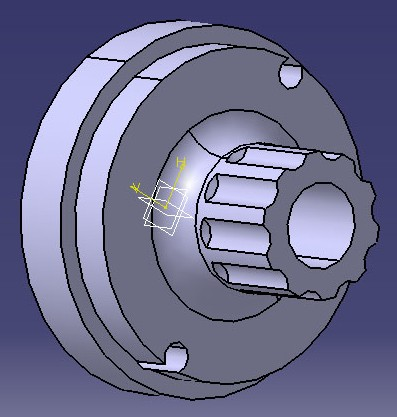
\includegraphics[scale=0.36]{images/CAD3D}
}

\subtitle{}
\author[Dr. Johannes Riesterer]
{Dr. rer. nat. Johannes Riesterer}

\date[KPT 2004]
{}

\maketitle


\begin{frame}
    \frametitle{Algorithmen und Datenstrukturen}
    \framesubtitle{Z-Buffer}
    \small
    \begin{block}{Grundidee}
    Der Z-Buffer speichert f\"ur jedes Pixel $(u,v)$ den Tiefenwert des aktuell
    n\"achsten sichtbaren Fragments. Beim Rasterisieren wird ein neues Fragment
    nur dann \"ubernommen, wenn sein Tiefenwert kleiner ist als der bisher
    gespeicherte Wert.
    \end{block}

    \begin{block}{Interpretation}
    In normierten Clipping-Koordinaten liegt der Tiefenwert typischerweise im
    Bereich $[-1,1]$. Der Z-Buffer l\"ost damit das Sichtbarkeitsproblem lokal
    pro Pixel und ersetzt teure globale Sortierungen von Polygonen.
    \end{block}

    \begin{align*}
    Z\text{-}Buffer : \mathbb{N} \times \mathbb{N} \to [-1,1]
    \end{align*}

    \begin{figure}
        \centering
        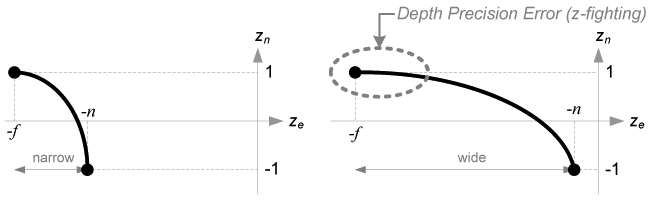
\includegraphics[width=0.82\textwidth]{images/gl_projectionmatrix_zbuffer_1.png}
        \caption{Z-Buffer-Wert pro Pixel}
        \label{fig:zbuffer-war}
    \end{figure}
\end{frame}


\begin{frame}
    \frametitle{Algorithmen und Datenstrukturen}
    \framesubtitle{Shadow Mapping}
    \small
    \begin{block}{Prinzip}
    Beim Shadow Mapping wird die Szene zun\"achst aus Sicht der Lichtquelle
    gerendert. Die dabei entstehende Tiefeninformation wird in einer Shadow Map
    gespeichert.
    \end{block}

    \begin{block}{Verwendung im zweiten Pass}
    Anschlie{\ss}end wird die Szene aus Kamerasicht gerendert. F\"ur jedes
    Fragment wird seine Position in den Koordinatenraum der Lichtquelle
    transformiert und mit dem in der Shadow Map gespeicherten Tiefenwert
    verglichen. Liegt das Fragment weiter entfernt als der gespeicherte Wert,
    befindet es sich im Schatten.
    \end{block}
\end{frame}


\begin{frame}
    \frametitle{Algorithmen und Datenstrukturen}
    \framesubtitle{Shadow Mapping}
    \begin{figure}
        \centering
        \subfloat[Tiefeninformation aus Sicht des Lichts]{
             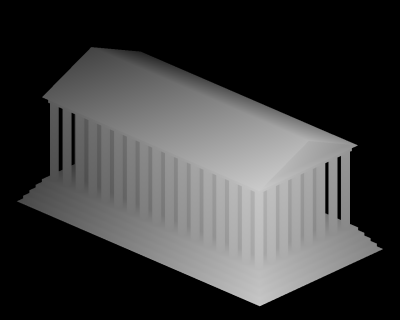
\includegraphics[width=0.35\textwidth]{images/sm_zb.png}
             \label{fig:shadowmap3}
        }
        \hspace*{0.08\textwidth}
        \subfloat[Rendering ohne Shadow Map]{
            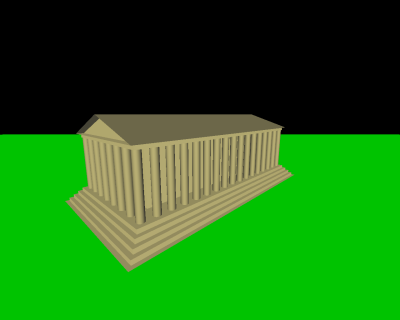
\includegraphics[width=0.35\textwidth]{images/sm_ns.png}
            \label{fig:shadowmap1}
        }

        \vspace*{1em}

        \subfloat[Rendering mit Shadow Map]{
             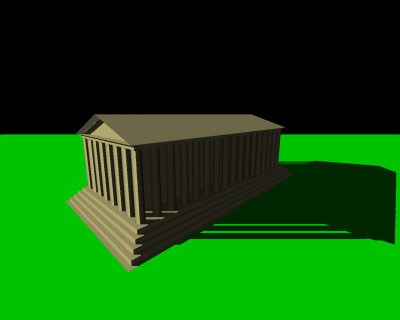
\includegraphics[width=0.35\textwidth]{images/sm_ws.png}
             \label{fig:shadowmap2}
        }
    \end{figure}
\end{frame}


\begin{frame}
    \frametitle{Algorithmen und Datenstrukturen}
    \framesubtitle{Texture Mapping}
    \small
    \begin{block}{Grundidee}
    Beim Texture Mapping werden Bilddaten auf eine Oberfl\"ache \"ubertragen.
    Dazu besitzt das Mesh zus\"atzliche 2D-Koordinaten im Texturraum, meist
    UV-Koordinaten genannt.
    \end{block}

    \begin{block}{Mathematische Sicht}
    Eine Texturabbildung ordnet Punkte einer 2D-Textur Punkten auf einer
    3D-Oberfl\"ache zu. Dadurch k\"onnen Farb- und Materialdetails dargestellt
    werden, ohne die Geometrie zu verfeinern.
    \end{block}

    \begin{align*}
    T : \mathbb{R}^2 \to \mathbb{R}^3
    \end{align*}

    \begin{figure}
        \centering
        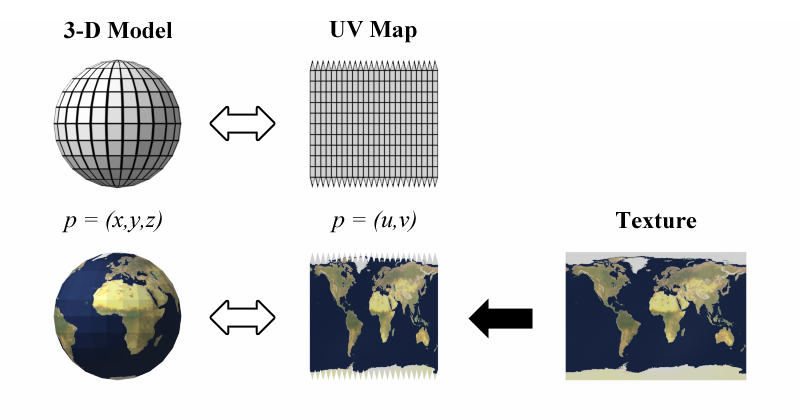
\includegraphics[width=0.72\textwidth]{images/tm_uv.png}
        \caption{UV-Mapping}
        \label{fig:uv-mapping1}
    \end{figure}
\end{frame}


\begin{frame}
    \frametitle{Algorithmen und Datenstrukturen}
    \framesubtitle{Texture Mapping}
    \small
    \begin{block}{Praktische Bedeutung}
    Gute UV-Koordinaten reduzieren Verzerrungen und sichtbare N\"ahte. Gerade
    bei Gesichtern oder komplexen Figuren ist das UV-Unwrapping ein wichtiger
    Modellierungsschritt.
    \end{block}

    \begin{figure}
        \centering
        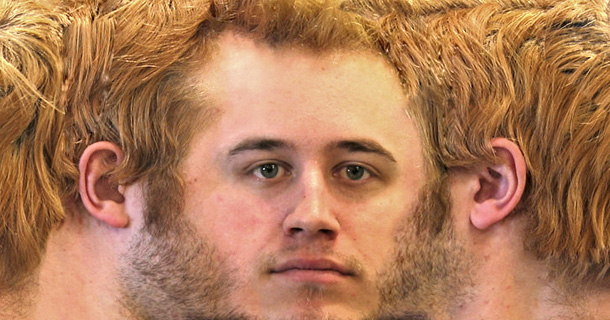
\includegraphics[width=0.95\textwidth]{images/tm_face.jpg}
        \caption{UV-Mapping auf einem Gesicht}
        \label{fig:uv-mapping2}
    \end{figure}
\end{frame}


\begin{frame}
    \frametitle{Algorithmen und Datenstrukturen}
    \framesubtitle{Bump Mapping}
    \small
    \begin{block}{Prinzip}
    Beim Bump Mapping werden relative H\"oheninformationen in einer Textur
    gespeichert. F\"ur die Beleuchtungsberechnung werden daraus lokal ver\"anderte
    Normalen abgeleitet.
    \end{block}

    \begin{block}{Wirkung}
    Die Oberfl\"ache wirkt feiner strukturiert, obwohl die zugrunde liegende
    Geometrie unver\"andert bleibt. Dadurch lassen sich kleine Details wie
    Poren, Kratzer oder Steinstrukturen sehr effizient darstellen.
    \end{block}

    \begin{figure}
        \centering
        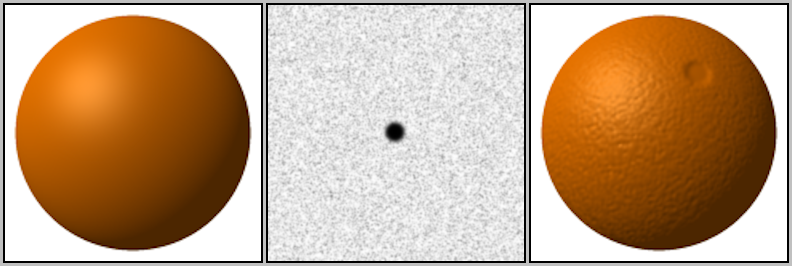
\includegraphics[width=0.78\textwidth]{images/Bumpmap.png}
        \caption{Bump Mapping}
    \end{figure}
\end{frame}


\begin{frame}
    \frametitle{Algorithmen und Datenstrukturen}
    \framesubtitle{Displacement Mapping}
    \small
    \begin{block}{Unterschied zum Bump Mapping}
    Auch hier wird eine Heightmap verwendet. Im Gegensatz zum Bump Mapping
    werden die Punkte des Gitternetzes jedoch tats\"achlich entlang ihrer
    Normalen verschoben.
    \end{block}

    \begin{block}{Folgen}
    Dadurch \"andert sich die echte Geometrie und nicht nur die Beleuchtung.
    Das Verfahren ist aufwendiger, liefert aber Silhouetten und Schatten, die
    zu den Oberfl\"achendetails passen.
    \end{block}

    \begin{figure}
        \centering
        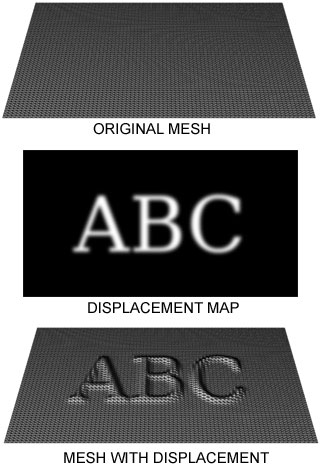
\includegraphics[width=0.20\textwidth]{images/Displacement.jpg}
        \caption{Displacement Mapping}
        \label{fig:displacement-mapping}
    \end{figure}

    \begin{figure}
        \centering
        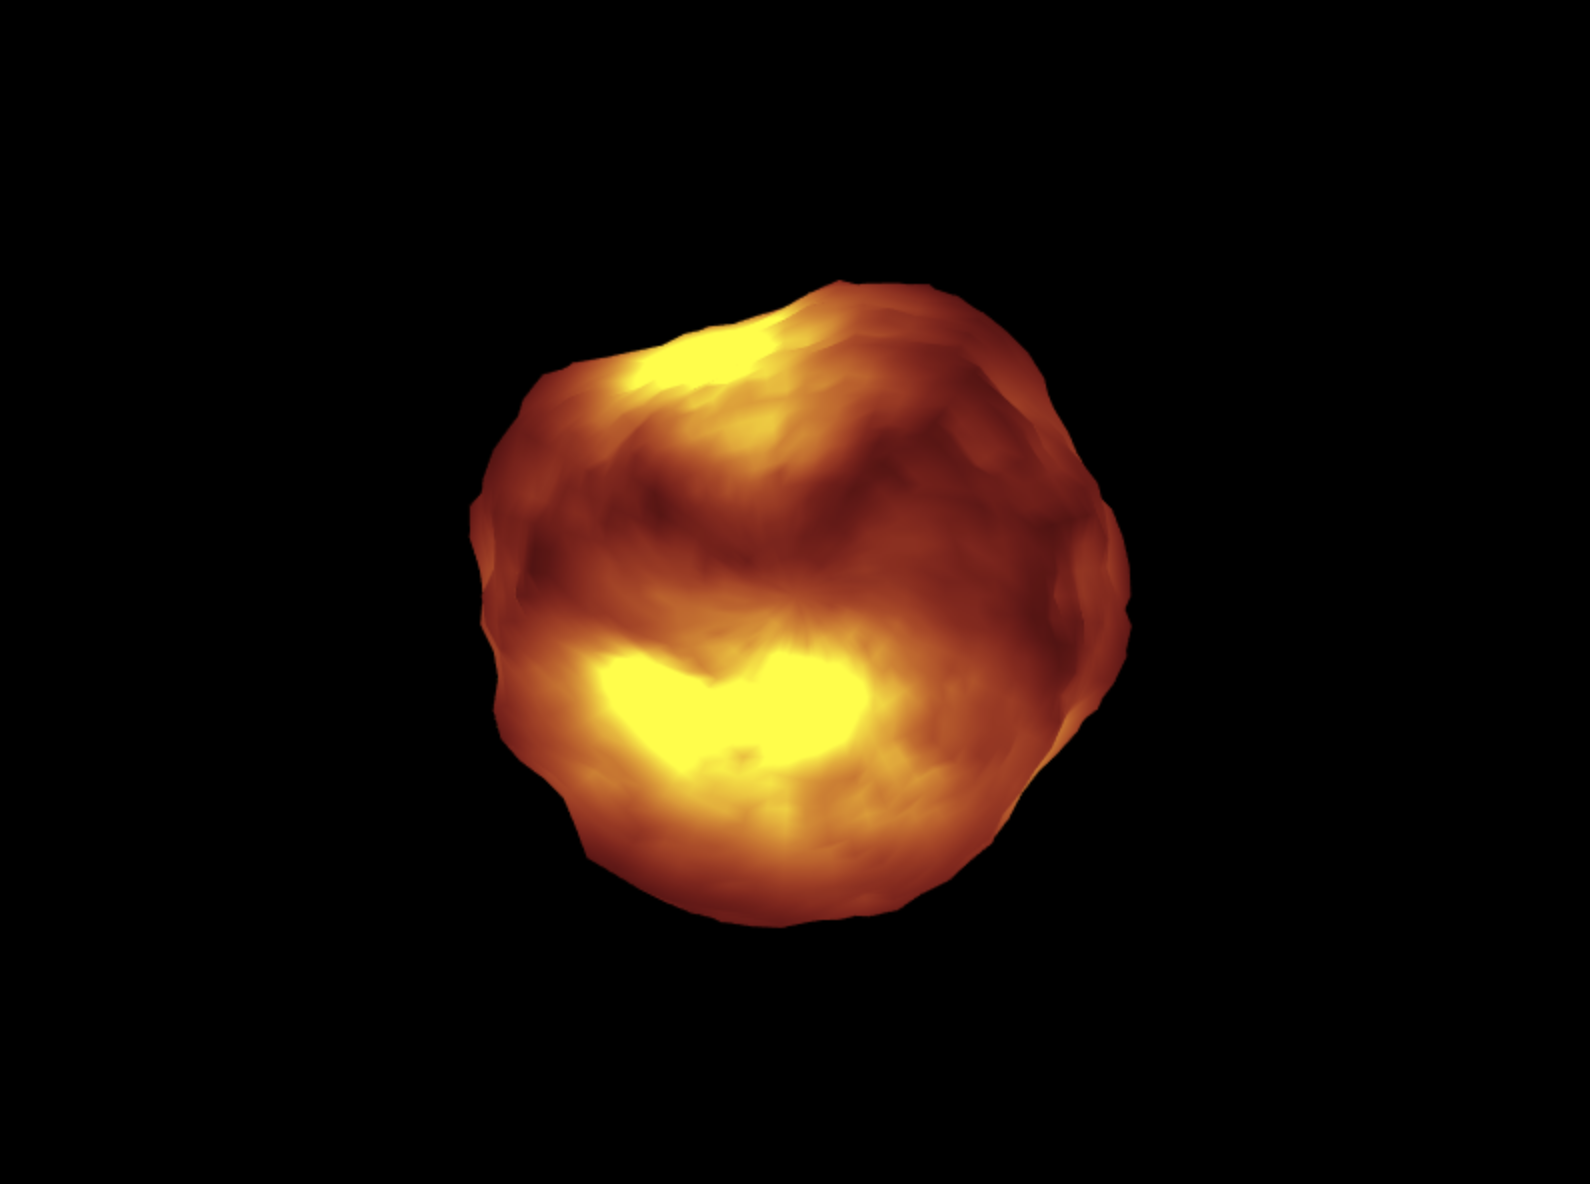
\includegraphics[width=0.28\textwidth]{images/lava.png}
        \caption{Beispiel mit ver\"anderter Geometrie}
        \label{fig:lava-ball}
    \end{figure}
\end{frame}


\begin{frame}
    \frametitle{Algorithmen und Datenstrukturen}
    \framesubtitle{Perlin Noise}
    \small
    \begin{block}{Grundidee}
    Perlin Noise ist ein Verfahren zur Erzeugung zuf\"alliger, aber glatter und
    organisch wirkender Muster. Entwickelt wurde der Ansatz von Ken Perlin, um
    nat\"urliche Strukturen wie Wolken, Rauch, Marmor oder Terrain synthetisch
    zu erzeugen.
    \end{block}

    \begin{block}{Eigenschaften}
    Im Gegensatz zu reinem Zufallsrauschen besitzt Perlin Noise lokale
    Koh\"arenz. Benachbarte Punkte haben also \"ahnliche Werte, wodurch
    kontinuierliche Strukturen entstehen.
    \end{block}
\end{frame}


\begin{frame}
    \frametitle{Algorithmen und Datenstrukturen}
    \framesubtitle{Perlin Noise}
    \begin{figure}
        \centering
        \subfloat[Anwendung von Perlin Noise]{
            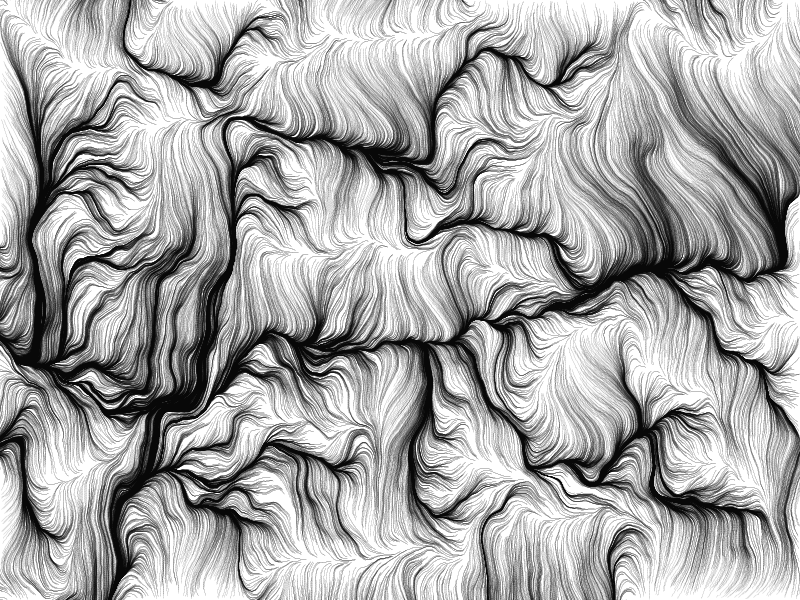
\includegraphics[width=0.4\textwidth]{images/perlinnoisepattern.png}
        }
        \hspace{1em}
        \subfloat[Terrain mit Perlin Noise]{
            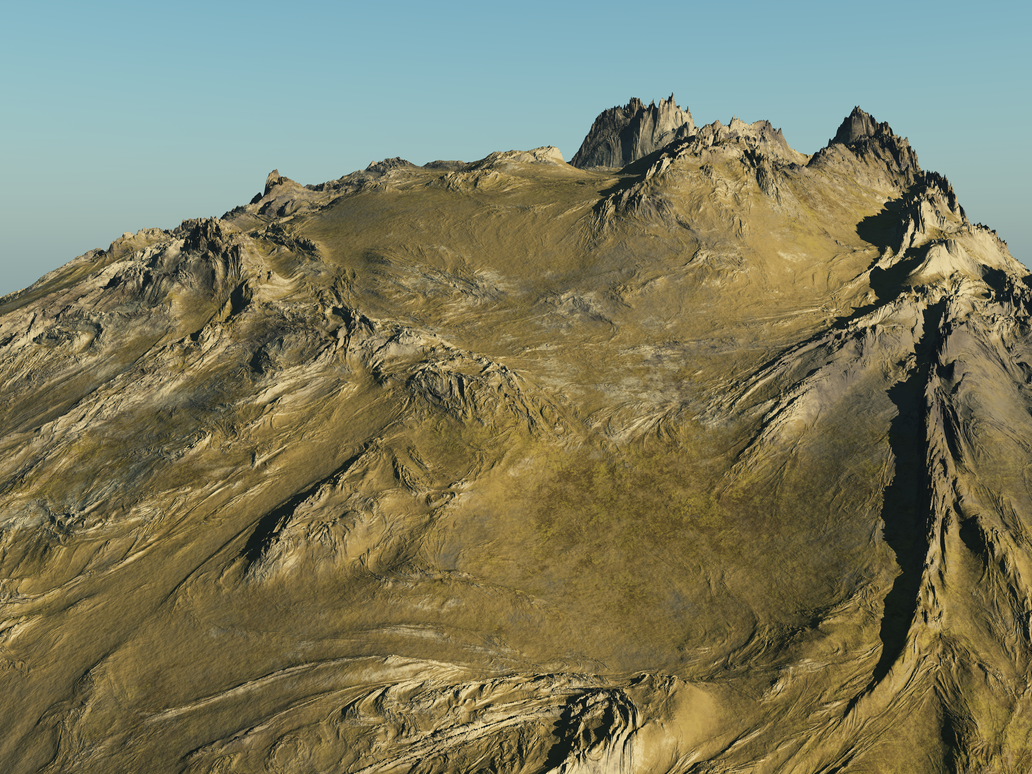
\includegraphics[width=0.4\textwidth]{images/terrain.png}
        }
    \end{figure}
\end{frame}


\begin{frame}
    \frametitle{Algorithmen und Datenstrukturen}
    \framesubtitle{Perlin Noise: Gradienten}
    \small
    \begin{block}{Schritt 1}
    An den Punkten eines regelm\"a{\ss}igen Gitters werden Zufallsvektoren
    erzeugt. Diese Vektoren definieren die lokale Richtung des Gradientenfeldes.
    \end{block}

    \begin{figure}
        \centering
        \includegraphics[width=0.75\textwidth]{images/perlinNoiseNV.png}
        \caption{Zufallsvektoren an Gitterpunkten}
    \end{figure}
\end{frame}


\begin{frame}
    \frametitle{Algorithmen und Datenstrukturen}
    \framesubtitle{Perlin Noise: Interpolation}
    \small
    \begin{block}{Schritt 2}
    F\"ur einen Punkt im Inneren einer Gitterzelle werden die Skalarprodukte
    zwischen Abstandsvektoren und den Gradienten an den Eckpunkten berechnet.
    Diese Werte werden anschlie{\ss}end glatt interpoliert.
    \end{block}

    \begin{block}{Ergebnis}
    So entsteht eine kontinuierliche Rauschfunktion, die in der Praxis oft
    \"uber mehrere Frequenzstufen kombiniert wird.
    \end{block}

    \begin{figure}
        \centering
        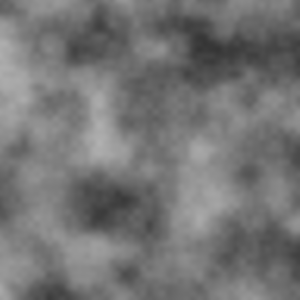
\includegraphics[width=0.35\textwidth]{images/perlin_noise.png}
        \caption{Perlin-Noise-Textur}
    \end{figure}
\end{frame}


\begin{frame}
    \frametitle{Algorithmen und Datenstrukturen}
    \framesubtitle{Kd-Trees}
    \small
    \begin{block}{Grundidee}
    Kd-Trees sind balancierte Bin\"arb\"aume f\"ur Punkte oder Objekte in einem
    $k$-dimensionalen Raum. Jede Ebene teilt den Raum durch eine Hyperebene
    orthogonal zu einer Koordinatenachse in zwei Teilr\"aume.
    \end{block}

    \begin{block}{Nutzen}
    Dadurch lassen sich Bereichsabfragen, N\"achste-Nachbarn-Suche oder
    Strahltests oft deutlich effizienter ausf\"uhren als mit einem linearen
    Vergleich aller Elemente.
    \end{block}

    \begin{figure}
        \centering
        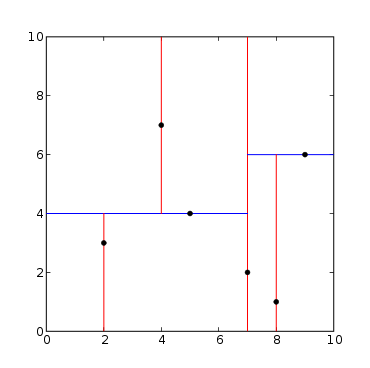
\includegraphics[width=0.25\textwidth]{images/kdtree_2d.png}
        \hspace{1em}
        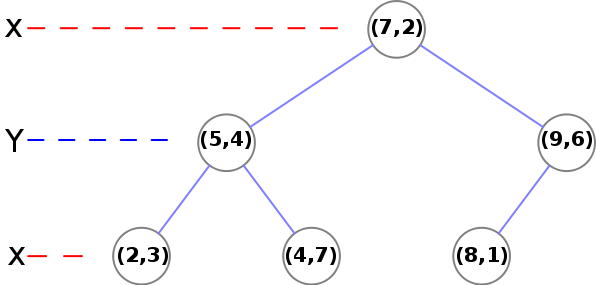
\includegraphics[width=0.25\textwidth]{images/kdtree.png}
    \end{figure}
\end{frame}


\begin{frame}
    \frametitle{Algorithmen und Datenstrukturen}
    \framesubtitle{Bounding Volume Hierarchies}
    \small
    \begin{block}{Grundidee}
    Eine Bounding Volume Hierarchy (BVH) ist ein Baum, in dem jeder innere
    Knoten eine einfache H\"ullgeometrie wie eine Axis-Aligned Bounding Box
    oder eine Kugel speichert. Diese H\"ulle umfasst alle Objekte des
    jeweiligen Teilbaums.
    \end{block}

    \begin{block}{Warum BVHs wichtig sind}
    \begin{itemize}
        \item Strahlverfolgung: Nur ein kleiner Teil aller Dreiecke muss exakt getestet werden.
        \item Picking und Kollision: Erst billige H\"ulltests, dann teure Exakttests.
        \item Sichtbarkeit: F\"ur Frustum Culling k\"onnen ganze Teilb\"aume verworfen werden.
    \end{itemize}
    \end{block}
\end{frame}
\begin{frame}
    \frametitle{Algorithmen und Datenstrukturen}
    \framesubtitle{Bounding Volume Hierarchies}
        \begin{figure}
        \centering
        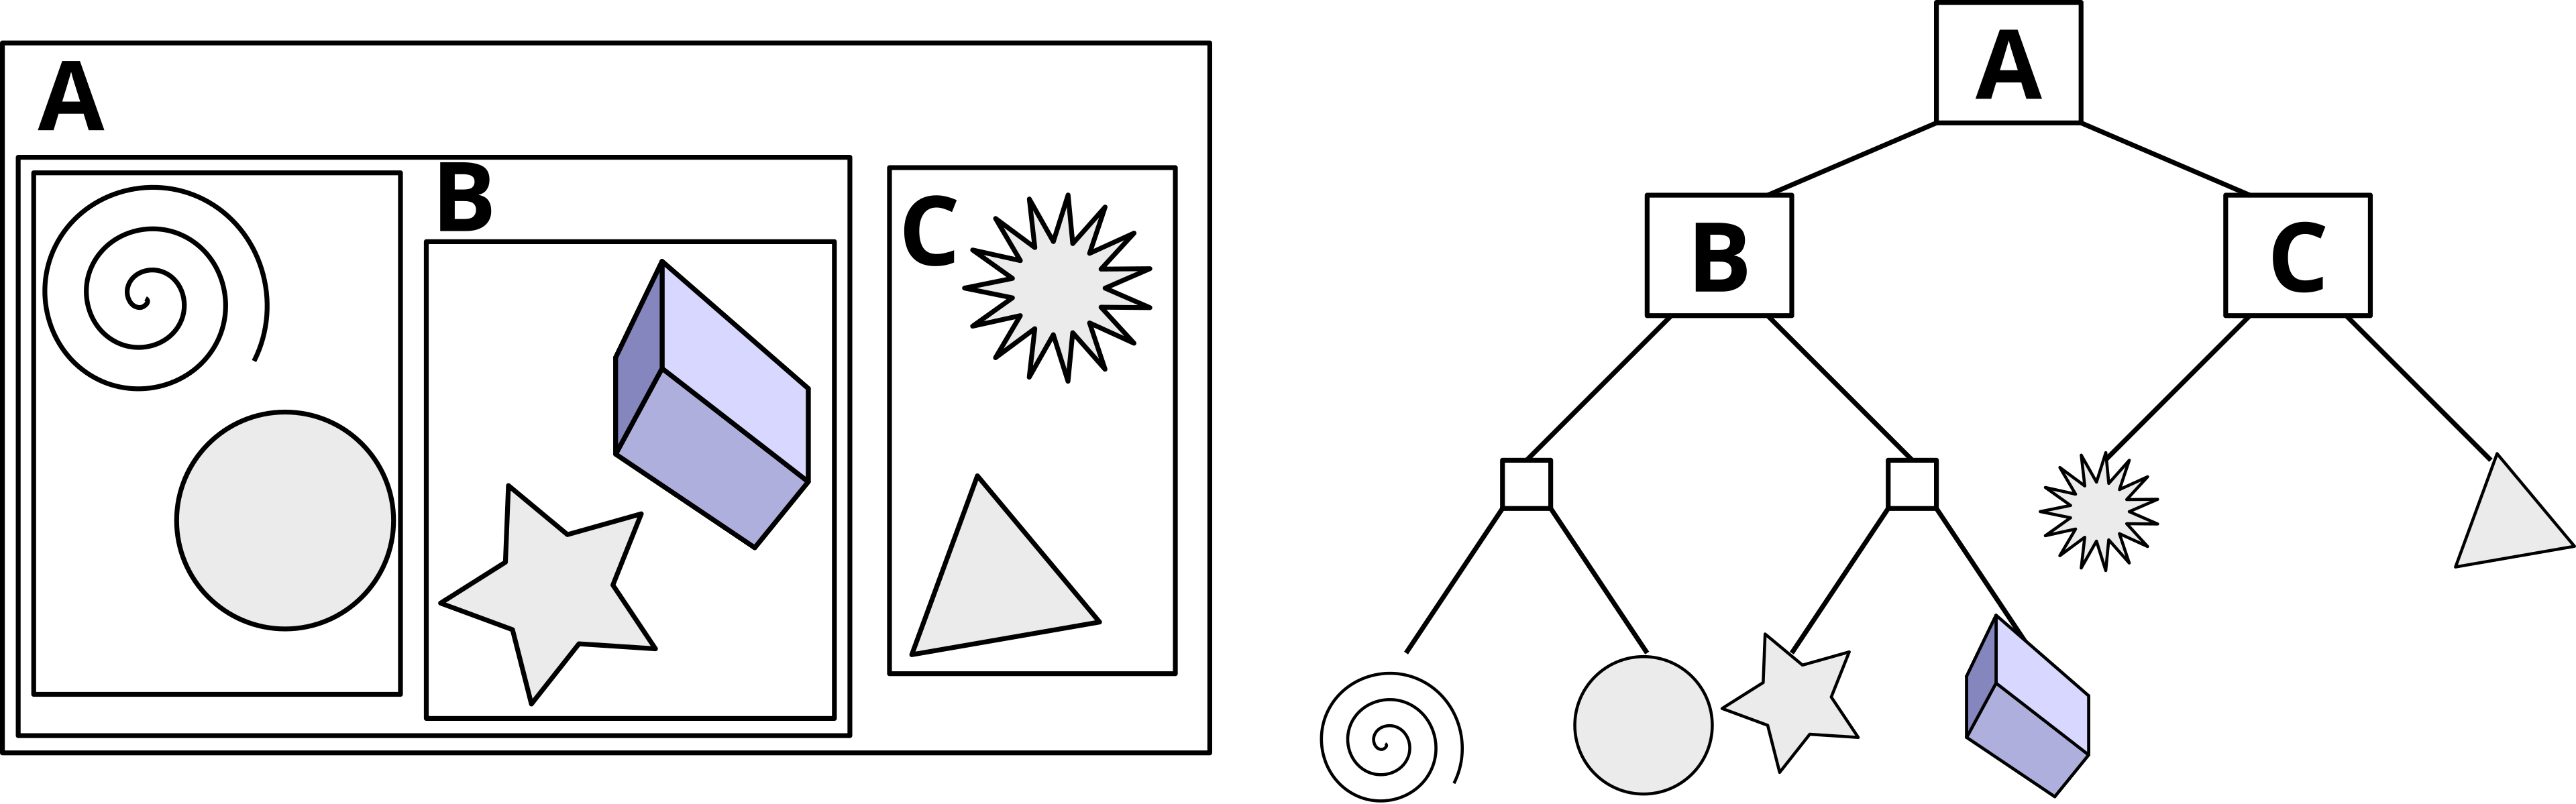
\includegraphics[width=0.9\textwidth]{images/bvh.png}
    \end{figure}
\end{frame}



\begin{frame}
    \frametitle{Algorithmen und Datenstrukturen}
    \framesubtitle{Bounding Volume Hierarchies}
    \small
    \begin{block}{Aufbau und Traversierung}
    Der Baum wird meist top-down aufgebaut, indem Geometrie entlang einer
    Raumachse oder mit einer Kostenfunktion wie der Surface Area Heuristic
    aufgeteilt wird. Bei einer Anfrage werden zuerst grobe H\"ullen getestet.
    Nur bei Treffer werden Teilb\"aume weiter traversiert oder einzelne
    Dreiecke untersucht.
    \end{block}

    \begin{block}{Faustregel}
    Je besser die H\"ullen angepasst sind und je ausgewogener der Baum ist,
    desto weniger primitive Tests sind bei Queries notwendig.
    \end{block}

\end{frame}


\begin{frame}
    \frametitle{Algorithmen und Datenstrukturen}
    \framesubtitle{Octrees}
    \small
    \begin{block}{Grundidee}
    Ein Octree zerlegt den dreidimensionalen Raum rekursiv in acht
    Teilw\"urfel. Leere oder homogene Bereiche werden grob gespeichert,
    nur komplexe Bereiche werden weiter verfeinert.
    \end{block}

    \begin{block}{Eigenschaften}
    \begin{itemize}
        \item Hierarchische Raumzerlegung statt Objektzerlegung
        \item Gute Repr\"asentation f\"ur Voxel- und Volumendaten
        \item Effizient bei gro{\ss}en leeren Bereichen
    \end{itemize}
    \end{block}
\end{frame}

\begin{frame}
    \frametitle{Algorithmen und Datenstrukturen}
    \framesubtitle{Octrees}
        \begin{figure}
        \centering
        \includegraphics[width=0.9\textwidth]{images/octree.png}
    \end{figure}
\end{frame}


\begin{frame}
    \frametitle{Algorithmen und Datenstrukturen}
    \framesubtitle{Octrees}
    \small
    \begin{block}{Operationen und Parameter}
    Einf\"ugen und Suchen folgen der Raumposition eines Objekts. Die maximale
    Tiefe des Baums bestimmt den r\"aumlichen Aufl\"osungsgrad und damit den
    Kompromiss zwischen Speicher, Genauigkeit und Traversierungskosten.
    \end{block}

    \begin{block}{Anwendungen}
    Voxelwelten, volumetrische Daten, Sichtbarkeitsabfragen, Kollision und
    Sparse Voxel Octrees f\"ur sehr gro{\ss}e Szenen.
    \end{block}
\end{frame}


\begin{frame}
    \frametitle{Algorithmen und Datenstrukturen}
    \framesubtitle{Half-Edge-Datenstruktur}
    \small
    \begin{block}{Motivation}
    Bei Polygonnetzen m\"ussen Nachbarschaften effizient traversiert werden:
    Welche Kanten grenzen an eine Fl\"ache? Welche Fl\"achen treffen sich an
    einer Kante? Welche Vertices liegen in der 1-Ring-Nachbarschaft?
    \end{block}
    \begin{block}{Struktur}
    Eine Kante wird in zwei gerichtete Halb-Kanten zerlegt. Jede Halb-Kante
    speichert typischerweise Referenzen auf Startvertex, Gegenkante, n\"achste
    Halb-Kante und zugeh\"orige Fl\"ache.
    \end{block}
        \begin{figure}
        \centering
        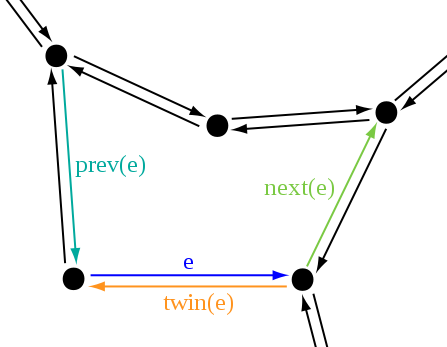
\includegraphics[width=0.4\textwidth]{images/halfedge.png}
    \end{figure}
\end{frame}



\begin{frame}
    \frametitle{Algorithmen und Datenstrukturen}
    \framesubtitle{Half-Edge-Datenstruktur}
    \small
    \begin{block}{Vorteile}
    Lokale topologische Operationen wie Split, Flip oder Collapse lassen sich
    direkt auf Zeigerstruktur-Ebene formulieren. Dadurch eignet sich die
    Struktur besonders f\"ur Mesh-Editing, Gl\"attung und Subdivision Surfaces.
    \end{block}

    \begin{block}{Wichtige Annahme}
    Besonders gut funktioniert die Struktur bei orientierten
    2-Mannigfaltigkeits-Meshes. Nicht-manigfaltige Kanten oder inkonsistente
    Orientierung machen den Umgang deutlich komplizierter.
    \end{block}
\end{frame}


\begin{frame}
    \frametitle{Algorithmen und Datenstrukturen}
    \framesubtitle{Mipmaps}
    \small
    \begin{block}{Grundidee}
    Mipmaps sind eine Hierarchie von Texturen mit abnehmender Aufl\"osung.
    Zu einer Textur der Gr\"o{\ss}e $w \times h$ werden verkleinerte Versionen
    mit etwa $\frac{w}{2} \times \frac{h}{2}$, $\frac{w}{4} \times \frac{h}{4}$
    usw. gespeichert.
    \end{block}

    \begin{block}{Nutzen}
    Mipmaps reduzieren Aliasing, verbessern die Cache-Lokalit\"at und
    beschleunigen die Filterung bei weit entfernten oder stark verkleinerten
    Objekten.
    \end{block}

\end{frame}


\begin{frame}
    \frametitle{Algorithmen und Datenstrukturen}
    \framesubtitle{Mipmaps}
    \small
    \begin{block}{Abtastung}
    Zur Laufzeit wird abh\"angig von der projizierten Texelgr\"o{\ss}e eine
    passende Ebene gew\"ahlt. Innerhalb einer Ebene spricht man von bilinearer
    Filterung, zwischen zwei benachbarten Ebenen von trilinearer Filterung.
    \end{block}

    \begin{block}{Trade-off}
    Mipmaps ben\"otigen zus\"atzlichen Speicher, reduzieren daf\"ur Flimmern
    und verbessern die Bildqualit\"at deutlich.
    \end{block}
\end{frame}


\begin{frame}
    \frametitle{Algorithmen und Datenstrukturen}
    \framesubtitle{Mipmaps: Intuition}
    \small
    \begin{block}{Warum reichen entfernten Objekten kleinere Texturen?}
    Ist ein Objekt weit entfernt, dann werden viele Texel der Originaltextur
    auf sehr wenige Bildschirmpixel projiziert. Ein einzelnes Pixel kann diese
    feinen Details nicht mehr getrennt darstellen.
    \end{block}

    \begin{block}{Problem ohne Mipmaps}
    Wenn trotzdem immer aus der vollen Aufl\"osung gesampelt wird, entstehen
    Flimmern, Moir\"e-Muster und unruhige Oberfl\"achen. Die Textur enth\"alt
    dann mehr Details, als auf dem Bildschirm sinnvoll dargestellt werden
    k\"onnen.
    \end{block}

    \begin{block}{Idee mit Mipmaps}
    Stattdessen verwendet man eine bereits verkleinerte Texturstufe, in der
    die feinen Details passend zusammengefasst sind.
    \end{block}
\end{frame}


\begin{frame}
    \frametitle{Algorithmen und Datenstrukturen}
    \framesubtitle{Mipmaps: Beispiel und Speicherbedarf}
    \small
    \begin{block}{Beispiel}
    Eine Textur mit $1024 \times 1024$ Pixeln besitzt zus\"atzlich Stufen mit
    $512 \times 512$, $256 \times 256$, $128 \times 128$ usw. Ein nahes Objekt
    nutzt eine feine Stufe, ein entferntes Objekt eine grobere Stufe.
    \end{block}

    \begin{block}{Filterung}
    Innerhalb einer Stufe werden benachbarte Texel interpoliert
    (bilineare Filterung). Liegt die passende Aufl\"osung zwischen zwei
    Stufen, wird auch zwischen diesen beiden Ebenen gemischt
    (trilineare Filterung).
    \end{block}

    \begin{block}{Speicheraufwand}
    Die gesamte Mipmap-Hierarchie ben\"otigt ungef\"ahr ein Drittel mehr
    Speicher als nur die Originaltextur, liefert daf\"ur aber deutlich
    stabilere und ruhigere Bilder.
    \end{block}
\end{frame}


\begin{frame}
    \frametitle{Algorithmen und Datenstrukturen}
    \framesubtitle{Level of Detail}
    \small
    \begin{block}{Grundidee}
    Bei Level-of-Detail-Verfahren wird dasselbe Objekt in mehreren Varianten
    unterschiedlicher Komplexit\"at gespeichert oder zur Laufzeit vereinfacht.
    \end{block}

    \begin{block}{Motivation}
    Nahe Objekte werden detailliert dargestellt, entfernte Objekte mit weniger
    Polygonen. Dadurch sinken Speicherbedarf, Speicherbandbreite und
    Rechenzeit.
    \end{block}

    \begin{block}{Auswahl der Stufe}
    Die Wahl kann auf Basis der Entfernung zur Kamera, der projizierten
    Bildschirmfl\"ache oder eines Fehlersch\"atzers erfolgen.
    \end{block}
\end{frame}


\begin{frame}
    \frametitle{Algorithmen und Datenstrukturen}
    \framesubtitle{LOD und Mesh Simplification}
    \small
    \begin{block}{Mesh Simplification}
    Eine typische Strategie f\"ur LOD ist die Vereinfachung eines Netzes durch
    lokale Operationen wie Edge Collapse. Dabei werden Vertices und Kanten
    schrittweise entfernt, w\"ahrend der geometrische Fehler klein bleibt.
    \end{block}

    \begin{block}{Bewertung}
    Der Vereinfachungsfehler kann \"uber Distanzma{\ss}e, Fl\"achenabweichungen
    oder Quadric Error Metrics abgesch\"atzt werden. Viele Systeme erzeugen
    daraus eine Folge verschachtelter Netze f\"ur diskrete oder kontinuierliche
    LOD-\"Uberg\"ange.
    \end{block}
\end{frame}


\begin{frame}
    \frametitle{Algorithmen und Datenstrukturen}
    \framesubtitle{Frustum Culling}
    \small
    \begin{block}{Grundidee}
    Vor dem Rendern wird gepr\"uft, ob ein Objekt \"uberhaupt im Sichtvolumen
    der Kamera liegt. Liegt seine Bounding Box vollst\"andig au{\ss}erhalb des
    View-Frustums, kann das Objekt verworfen werden.
    \end{block}

    \begin{block}{Nutzen}
    Frustum Culling spart Vertex- und Fragmentarbeit und wird oft mit BVHs,
    Octrees oder Bounding Spheres kombiniert.
    \end{block}
\end{frame}


\begin{frame}
    \frametitle{Algorithmen und Datenstrukturen}
    \framesubtitle{Frustum Culling}
    \small
    \begin{block}{Geometrische Idee}
    Das Sichtvolumen der Kamera wird durch sechs Ebenen beschrieben: links,
    rechts, oben, unten, near und far. F\"ur jedes Objekt wird getestet, auf
    welcher Seite dieser Ebenen seine H\"ulle liegt.
    \end{block}

    \begin{block}{Ablauf in der Praxis}
    \begin{itemize}
        \item Teste zuerst eine einfache H\"ulle wie Kugel oder AABB.
        \item Verwirf das Objekt sofort, wenn es au{\ss}erhalb einer Ebene liegt.
        \item Traversiere bei Hierarchien nur die Teilb\"aume, deren H\"ulle sichtbar ist.
    \end{itemize}
    \end{block}
\end{frame}




\begin{frame}
    \frametitle{Algorithmen und Datenstrukturen}
    \framesubtitle{Spatial Hashing}
    \small
    \begin{block}{Grundidee}
    Spatial Hashing kombiniert ein gedachtes Uniform Grid mit einer
    Hash-Tabelle. Der Raum wird in Zellen gleicher Gr\"o{\ss}e zerlegt,
    aber nur tats\"achlich belegte Zellen werden gespeichert.
    \end{block}

    \begin{block}{Diskretisierung}
    F\"ur einen Punkt \(p=(x,y,z)\) und Zellgr\"o{\ss}e \(h\) ergibt sich
    die Gitterzelle
    \[
    i = \left\lfloor \frac{x}{h} \right\rfloor,\qquad
    j = \left\lfloor \frac{y}{h} \right\rfloor,\qquad
    k = \left\lfloor \frac{z}{h} \right\rfloor.
    \]
    Die ganzzahligen Zellkoordinaten werden anschlie{\ss}end auf einen
    Bucket der Hash-Tabelle abgebildet.
    \end{block}
\end{frame}


\begin{frame}
    \frametitle{Algorithmen und Datenstrukturen}
    \framesubtitle{Spatial Hashing}
    \small
    \begin{block}{Hashfunktion}
    Eine typische Hashfunktion f\"ur Zellkoordinaten lautet
    \[
    H(i,j,k) =
    (73856093\,i \oplus 19349663\,j \oplus 83492791\,k)\bmod M
    \]
    mit Tabellengr\"o{\ss}e \(M\). Mehrere Zellen k\"onnen auf denselben
    Bucket fallen und werden dann als Liste gespeichert.
    \end{block}

    \begin{block}{Beispiel}
    Bei Zellgr\"o{\ss}e \(h=1\) liegt der Punkt
    \(p=(2.3,1.7,-0.2)\) in der Zelle
    \[
    (2,1,-1).
    \]
    F\"ur eine Nachbarsuche m\"ussen dann nur die benachbarten Zellen
    betrachtet werden, nicht der gesamte Raum.
    \end{block}
\end{frame}


\begin{frame}
    \frametitle{Algorithmen und Datenstrukturen}
    \framesubtitle{Marching Cubes}
    \small
    \begin{block}{Volumendaten zu Dreiecksnetzen}
    Marching Cubes extrahiert aus einem skalarwertigen 3D-Gitter eine
    Isosurface zum Isolevel \(\tau\). Dazu wird jeder Gitterw\"urfel separat
    betrachtet und anhand seiner acht Eckwerte klassifiziert.
    \end{block}

    \begin{block}{Anwendungsbeispiele}
    Typische Quellen sind CT- und MRT-Daten, Dichtefelder,
    Fluidsimulationen oder implizite Fl\"achen. Das Ergebnis ist ein
    Dreiecksnetz, das sich mit klassischen Rendering-Pipelines effizient
    darstellen l\"asst.
    \end{block}
\end{frame}


\begin{frame}
    \frametitle{Algorithmen und Datenstrukturen}
    \framesubtitle{Marching Cubes: Voxelgitter}
    \begin{figure}
        \centering
        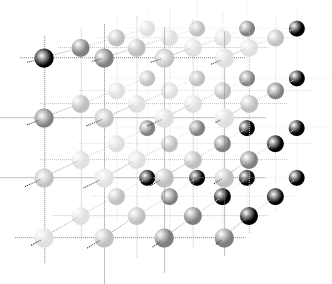
\includegraphics[width=0.4\textwidth]{images/Voxelgitter.png}
        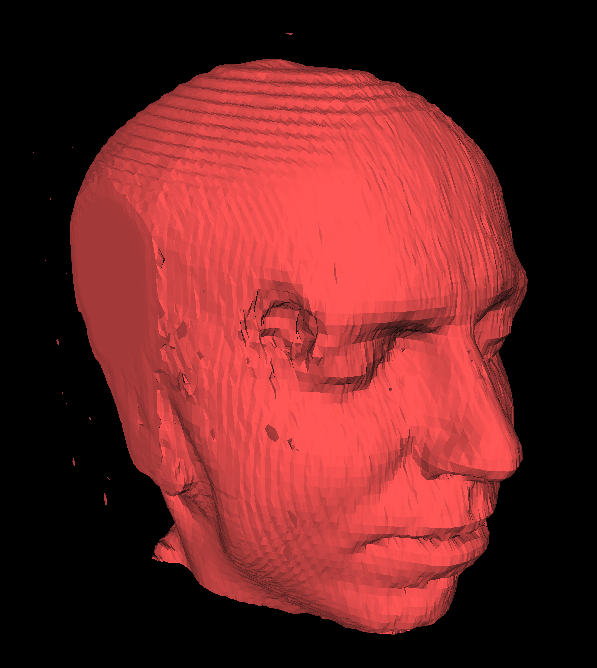
\includegraphics[width=0.4\textwidth]{images/marchingcubes_head.png}
    \end{figure}
    
\end{frame}


\begin{frame}
    \frametitle{Algorithmen und Datenstrukturen}
    \framesubtitle{Marching Cubes: Bitmaske}
    \small
    \begin{block}{Cube Mask / Cube Index}
    Jede der acht W\"urfelecken erh\"alt ein Bit:
    \[
    b_i =
    \begin{cases}
    1 & \text{falls } f(v_i) \geq \tau \\
    0 & \text{falls } f(v_i) < \tau
    \end{cases}
    \]
    Die Wahl dieser Konvention ist prinzipiell beliebig, muss aber f\"ur alle
    W\"urfel konsistent beibehalten werden. Daraus entsteht ein 8-Bit-Muster und
    damit ein Fallindex
    \[
    \texttt{cubeIndex} = \sum_{i=0}^{7} b_i 2^i
    \]
    mit insgesamt \(2^8 = 256\) m\"oglichen W\"urfelkonfigurationen.
    \end{block}
\end{frame}


\begin{frame}
    \frametitle{Algorithmen und Datenstrukturen}
    \framesubtitle{Marching Cubes: Bitmaske}
    \begin{figure}
        \centering
        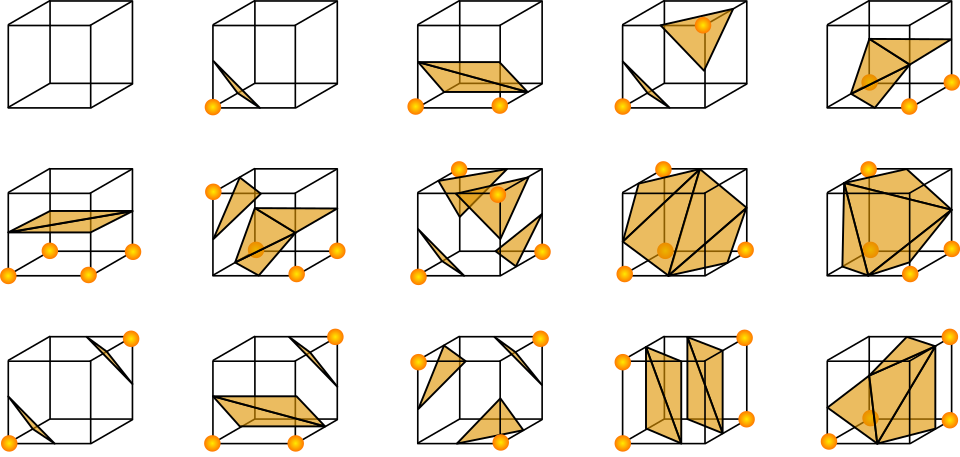
\includegraphics[width=0.7\textwidth]{images/marchingcubes_bit.png}
    \end{figure}
\end{frame}


\begin{frame}
    \frametitle{Algorithmen und Datenstrukturen}
    \framesubtitle{Marching Cubes: Kanten und Schnittpunkte}
    \small
    \begin{block}{Welche Kanten werden geschnitten?}
    Ein W\"urfel besitzt 12 Kanten. Eine Kante wird genau dann von der
    Isosurface geschnitten, wenn ihre beiden Endpunkte auf verschiedenen
    Seiten des Isolevels liegen, also unterschiedliche Bits besitzen.
    \end{block}

    \begin{block}{Interpolation}
    Der Schnittpunkt auf einer geschnittenen Kante zwischen \(p_1\) und
    \(p_2\) mit Skalarwerten \(f_1\) und \(f_2\) wird linear interpoliert:
    \[
    t = \frac{\tau - f_1}{f_2 - f_1},
    \qquad
    p = p_1 + t (p_2 - p_1)
    \]
    Liegen alle acht Ecken auf derselben Seite des Isolevels, entsteht
    kein Dreieck.
    \end{block}
\end{frame}


\begin{frame}
    \frametitle{Algorithmen und Datenstrukturen}
    \framesubtitle{Marching Cubes: Lookup-Tabelle}
    \small
    \begin{block}{Von der Bitmaske zu Dreiecken}
    Der \texttt{cubeIndex} adressiert in der Praxis zwei Lookup-Tabellen:
    \begin{itemize}
        \item eine Tabelle, die angibt, welche der 12 Kanten geschnitten werden,
        \item und eine Triangulationstabelle, die festlegt, wie die
        interpolierten Schnittpunkte zu Dreiecken verbunden werden.
    \end{itemize}
    Die Dreiecke werden also nicht frei konstruiert, sondern aus einer
    vordefinierten Falltabelle gelesen.
    \end{block}

    \begin{block}{Topologische Idee}
    Die Isosurface trennt Ecken mit \(f(v_i) < \tau\) von Ecken mit
    \(f(v_i) \geq \tau\). Marching Cubes approximiert diese Trennfl\"ache lokal
    innerhalb jedes W\"urfels durch ein oder mehrere Dreiecke.
    \end{block}
\end{frame}


\begin{frame}
    \frametitle{Algorithmen und Datenstrukturen}
    \framesubtitle{Marching Cubes: Einfacher Fall}
    \small
    \begin{block}{Beispielkonfiguration}
    Liegt genau eine W\"urfelecke auf einer Seite des Isolevels und die anderen
    sieben auf der anderen Seite, dann werden genau die drei an dieser Ecke
    anliegenden Kanten geschnitten.
    \end{block}

    \begin{block}{Folge}
    Die drei interpolierten Schnittpunkte bilden genau ein Dreieck. Dieser Fall
    zeigt anschaulich, wie aus einer lokalen Bitkonfiguration eine konkrete
    Polygonisierung entsteht.
    \end{block}
\end{frame}


\begin{frame}
    \frametitle{Algorithmen und Datenstrukturen}
    \framesubtitle{Marching Cubes: Ablauf pro W\"urfel}
    \small
    \begin{block}{Algorithmus}
    \begin{enumerate}
        \item Acht Eckwerte mit dem Isolevel vergleichen
        \item Bitmaske und \texttt{cubeIndex} berechnen
        \item Geschnittene Kanten aus der Lookup-Tabelle bestimmen
        \item Schnittpunkte auf den Kanten interpolieren
        \item Punkte gem\"a\ss{} Falltabelle zu Dreiecken verbinden
    \end{enumerate}
    \end{block}

    \begin{block}{St\"arken und Grenzen}
    Das Verfahren ist lokal, parallelisierbar und gut f\"ur regul\"are Gitter
    geeignet. Schwierigkeiten entstehen bei mehrdeutigen F\"allen, bei denen
    mehrere topologisch unterschiedliche Triangulierungen m\"oglich sind, sowie
    bei geringer Aufl\"osung oder verrauschten Daten.
    \end{block}
\end{frame}


\begin{frame}
    \frametitle{Algorithmen und Datenstrukturen}
    \framesubtitle{Marching Cubes: Interaktive Demo}
    \small
    \begin{block}{Beispiel}
    Interaktive Visualisierung des Verfahrens:
    \href{https://threejs.org/examples/webgl_marchingcubes.html}{threejs marching cubes example}
    \end{block}
\end{frame}


\begin{frame}
    \frametitle{Algorithmen und Datenstrukturen}
    \framesubtitle{Catmull-Clark-Subdivision}
    \small
    \begin{block}{Grundidee}
    Catmull-Clark ist ein Subdivision-Verfahren f\"ur Polygonnetze,
    insbesondere f\"ur Quad-Netze. In jedem Verfeinerungsschritt werden
    neue Fl\"achenpunkte, Kantenpunkte und verschobene Vertexpunkte berechnet.
    Dadurch entsteht aus einem groben Kontrollnetz schrittweise eine glatte
    Grenzfl\"ache.
    \end{block}


\end{frame}




\begin{frame}
    \frametitle{Algorithmen und Datenstrukturen}
    \framesubtitle{Catmull-Clark-Subdivision}
    \begin{block}{Neue Punkte}
    F\"ur eine Fl\"ache mit Vertices \(v_1,\dots,v_m\) gilt
    \[
    F = \frac{1}{m}\sum_{i=1}^m v_i
    \]
    f\"ur den Fl\"achenpunkt. F\"ur eine Kante mit Endpunkten \(v_1,v_2\)
    und benachbarten Fl\"achenpunkten \(F_1,F_2\) gilt
    \[
    E = \frac{v_1 + v_2 + F_1 + F_2}{4}.
    \]
    \end{block}

    \begin{figure}
        \centering
        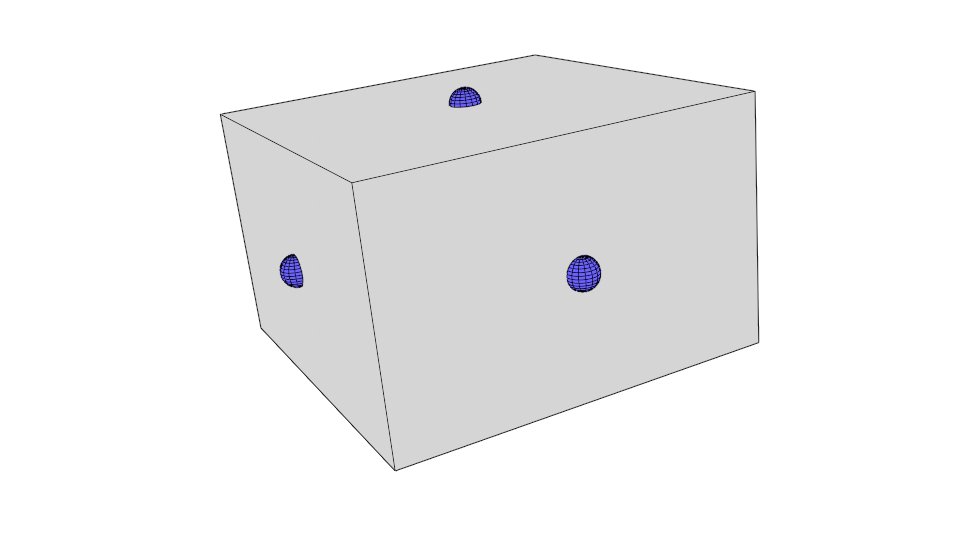
\includegraphics[width=0.3\textwidth]{images/Catmull-Clark_Recursive_Step_1}
        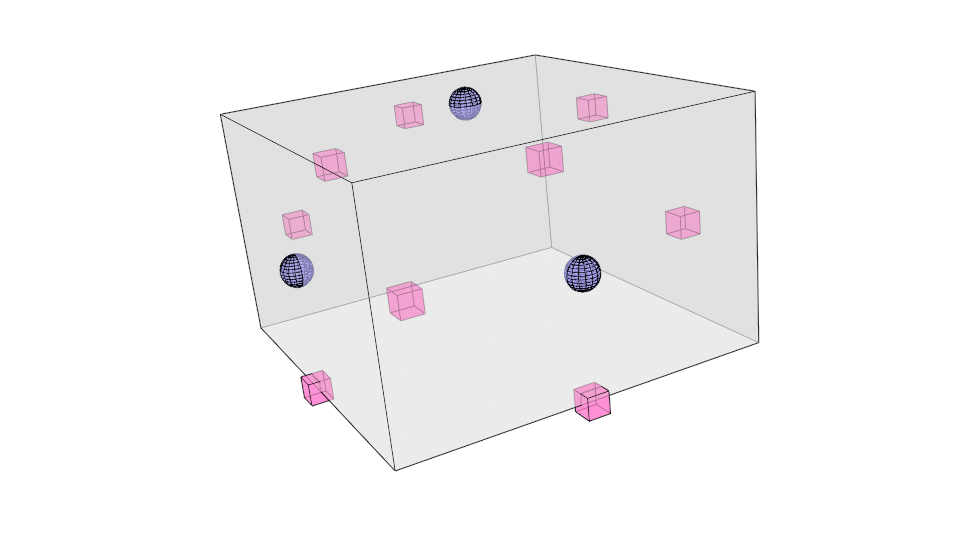
\includegraphics[width=0.3\textwidth]{images/Catmull-Clark_Recursive_Step_2}
    \end{figure}
\end{frame}



\begin{frame}
    \frametitle{Algorithmen und Datenstrukturen}
    \framesubtitle{Catmull-Clark-Subdivision}
    \small
    \begin{block}{Vertex-Regel}
    Sei \(n\) die Valenz eines Vertex \(P\), \(F\) der Mittelwert der
    benachbarten Fl\"achenpunkte und \(R\) der Mittelwert der Mittelpunkte
    benachbarter Kanten. Dann wird der Vertex verschoben zu
    \[
    P' = \frac{F + 2R + (n-3)P}{n}.
    \]
    \end{block}

    \begin{figure}
        \centering
        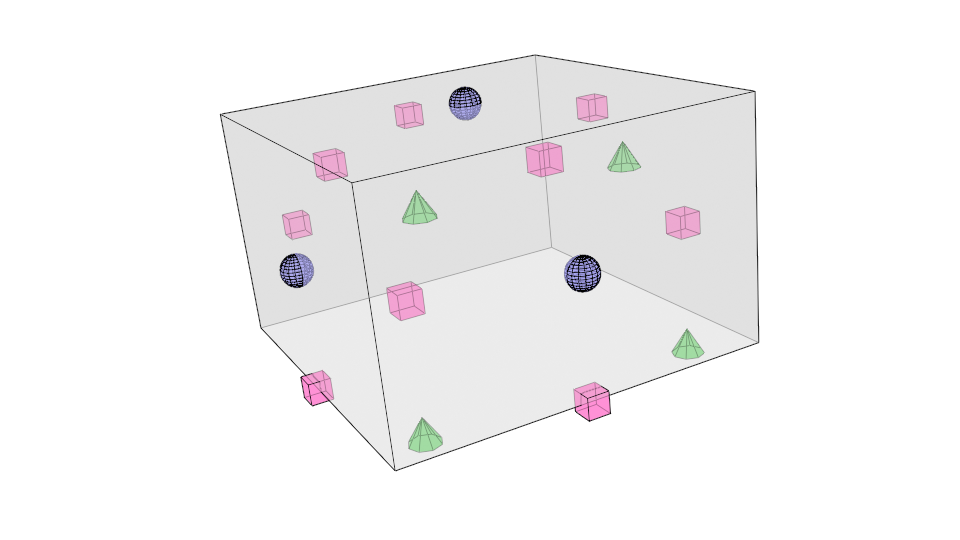
\includegraphics[width=0.3\textwidth]{images/Catmull-Clark_Recursive_Step_3}
    \end{figure}

\end{frame}


\begin{frame}
    \frametitle{Algorithmen und Datenstrukturen}
    \framesubtitle{Catmull-Clark-Subdivision}


    \begin{block}{Eigenschaften}
    Ein Quad wird in der Regel in vier kleinere Quads zerlegt. Nach
    wiederholter Anwendung entsteht eine glatte Fl\"ache. Bei regul\"aren
    Quad-Netzen ist die Grenzfl\"ache eng mit bicubischen B-Splines verwandt.
    \end{block}



    \begin{figure}
        \centering
        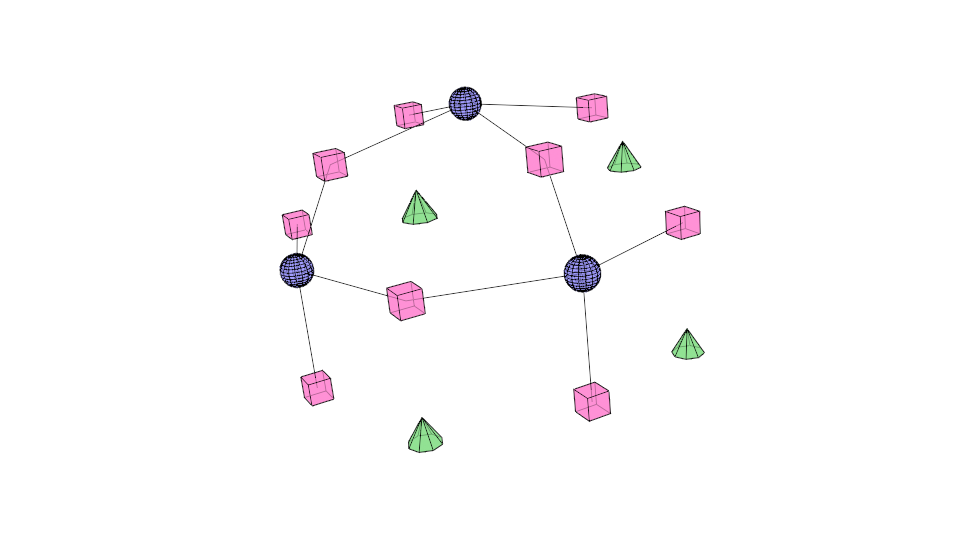
\includegraphics[width=0.3\textwidth]{images/Catmull-Clark_Recursive_Step_4}
                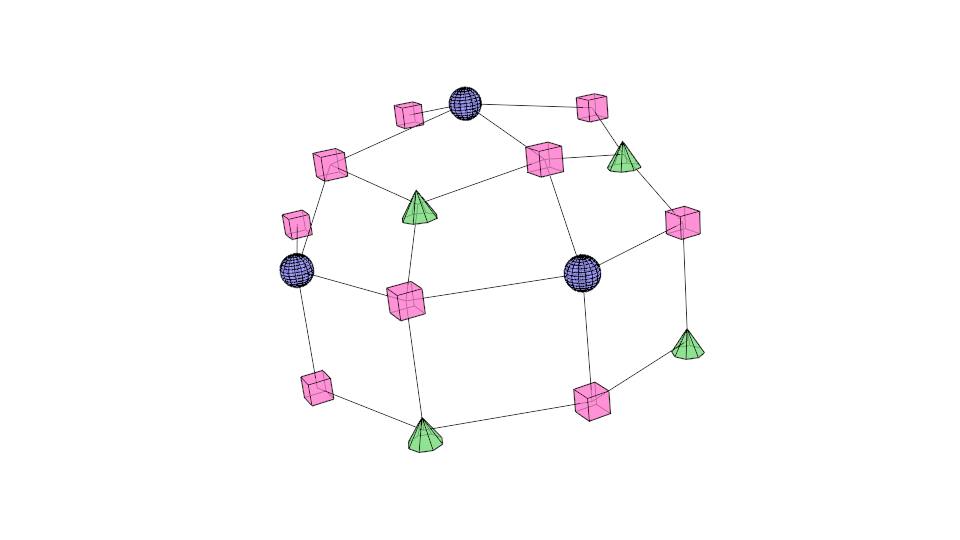
\includegraphics[width=0.3\textwidth]{images/Catmull-Clark_Recursive_Step_5}

    \end{figure}

\end{frame}

\end{document}